\chapter{The ATLAS Experiment}\label{chapter:ATLAS}

\section{Overview}\label{sec:ATLAS_overview}

The ATLAS Experiment~\cite{PERF-2007-01} is one of the four main LHC experiments with the ATLAS detector, seen in \Cref{fig:ATLAS_detector}, located in the experiment cavern at Point 1 of the LHC roughly $100~\textrm{m}$ underground.
The ATLAS detector, henceforth also referred to as just ``ATLAS,'' is a general purpose, high luminosity particle physics detector designed to be able to search for as many types of interesting physics events as possible.
ATLAS is the largest of the LHC experiments with dimensions of $44~\mathrm{m}$ in length and $25~\mathrm{m}$ in height.

\begin{figure}[htbp]
 \centering
 \includegraphics[width=0.9\textwidth]{ATLAS/ATLAS_detector.eps}
 \caption[Cut-away view of the ATLAS detector.]{%
  Model of human particle physicists with ATLAS detector shown for scale~\cite{Pequenao:1095924}.}\label{fig:ATLAS_detector}
\end{figure}

\section{Geometry}\label{sec:ATLAS_geometry}

The ATLAS detector is cylindrical in design and forward-backward symmetrical with respect to the center of the detector.
The inner detector is surrounded by a $2~\mathrm{T}$ superconducting solenoid magnet and provides excellent tracking coverage in $\abs{\eta} < 2.5$.
The inner detector is further bracketed at each end by end-cap toroid magnets and the entire barrel of the detector out through the calorimeters is enclosed in a toroid magnet system.
These two toroid systems are both constructed such that they exhibit an eight-fold azimuthal symmetry.
As a result, almost all of ATLAS also exhibits this eight-fold axial symmetry, with the noted exception of the support structures on the bottom that support the detector off the ground.
The detectors subsytems, described in the following sections, are radially concentric and cover different pseudorapidity ranges, with the liquid-argon (LAr) forward calorimeters extending the coverage out to $\abs{\eta} = 4.9$.

\section{Tracking in the Inner Detector}\label{sec:ATLAS_ID}

Located at the heart of ATLAS and inside of the $2~\mathrm{T}$ solenoidal magnetic field, the \gls{inner detector} subsystem, seen in \Cref{fig:ATLAS_inner_detector}, provides precision tracking through the combined performance of successive layers of pixel detectors, silicon \gls{SCT}, and the straw tube \gls{TRT} and provides excellent coverage up to $\abs{\eta} < 2.5$.
To maximize the effective detector area, the pixels and SCT in the barrel region are arranged in concentric cylinders, as seen in \Cref{fig:ATLAS_pixel}.
The pixel layers are closest to the beamline and consist of roughly $80.4$ million identical pixel sensors forming three cylindrical layers in the barrel and three consecutive disks at each end-cap.
Each of the pixels is of area\footnote{$50~\mu\mathrm{m}$ in the $R\textrm{-}\phi$ direction by $400~\mu\mathrm{m}$ in the $z$ direction.} $20,000~\mu\mathrm{m}^{2}$ with resolution of $10~\mu\mathrm{m}~(R\textrm{-}\phi) \times 115~\mu\mathrm{m}~(z)$.
The excellent resolution in $R\textrm{-}\phi$ is a result of the strong magnetic field bending particles along $\hat{\vec{\phi}}$ causing them to spiral through the pixel detector~\cite{PERF-2007-01}.
Charged particle hits in the pixel detector are paramount for robust tracking and identifying and reconstructing the primary and secondary vertices necessary for physics object reconstruction (i.e., jets) and flavor tagging.

\begin{figure}[htbp]
 \centering
 \includegraphics[width=0.65\textwidth]{ATLAS/ATLAS_inner_detector.eps}
 \caption[Cut-away view of the ATLAS inner detector showing the pixel detector, Semiconductor Tracker, and Transition Radiation Tracker.]{%
  Cut-away view of the ATLAS inner detector showing the pixel detector, Semiconductor Tracker, and Transition Radiation Tracker~\cite{Pequenao:1095926}.}\label{fig:ATLAS_inner_detector}
\end{figure}

\begin{figure}[htbp]
 \centering
 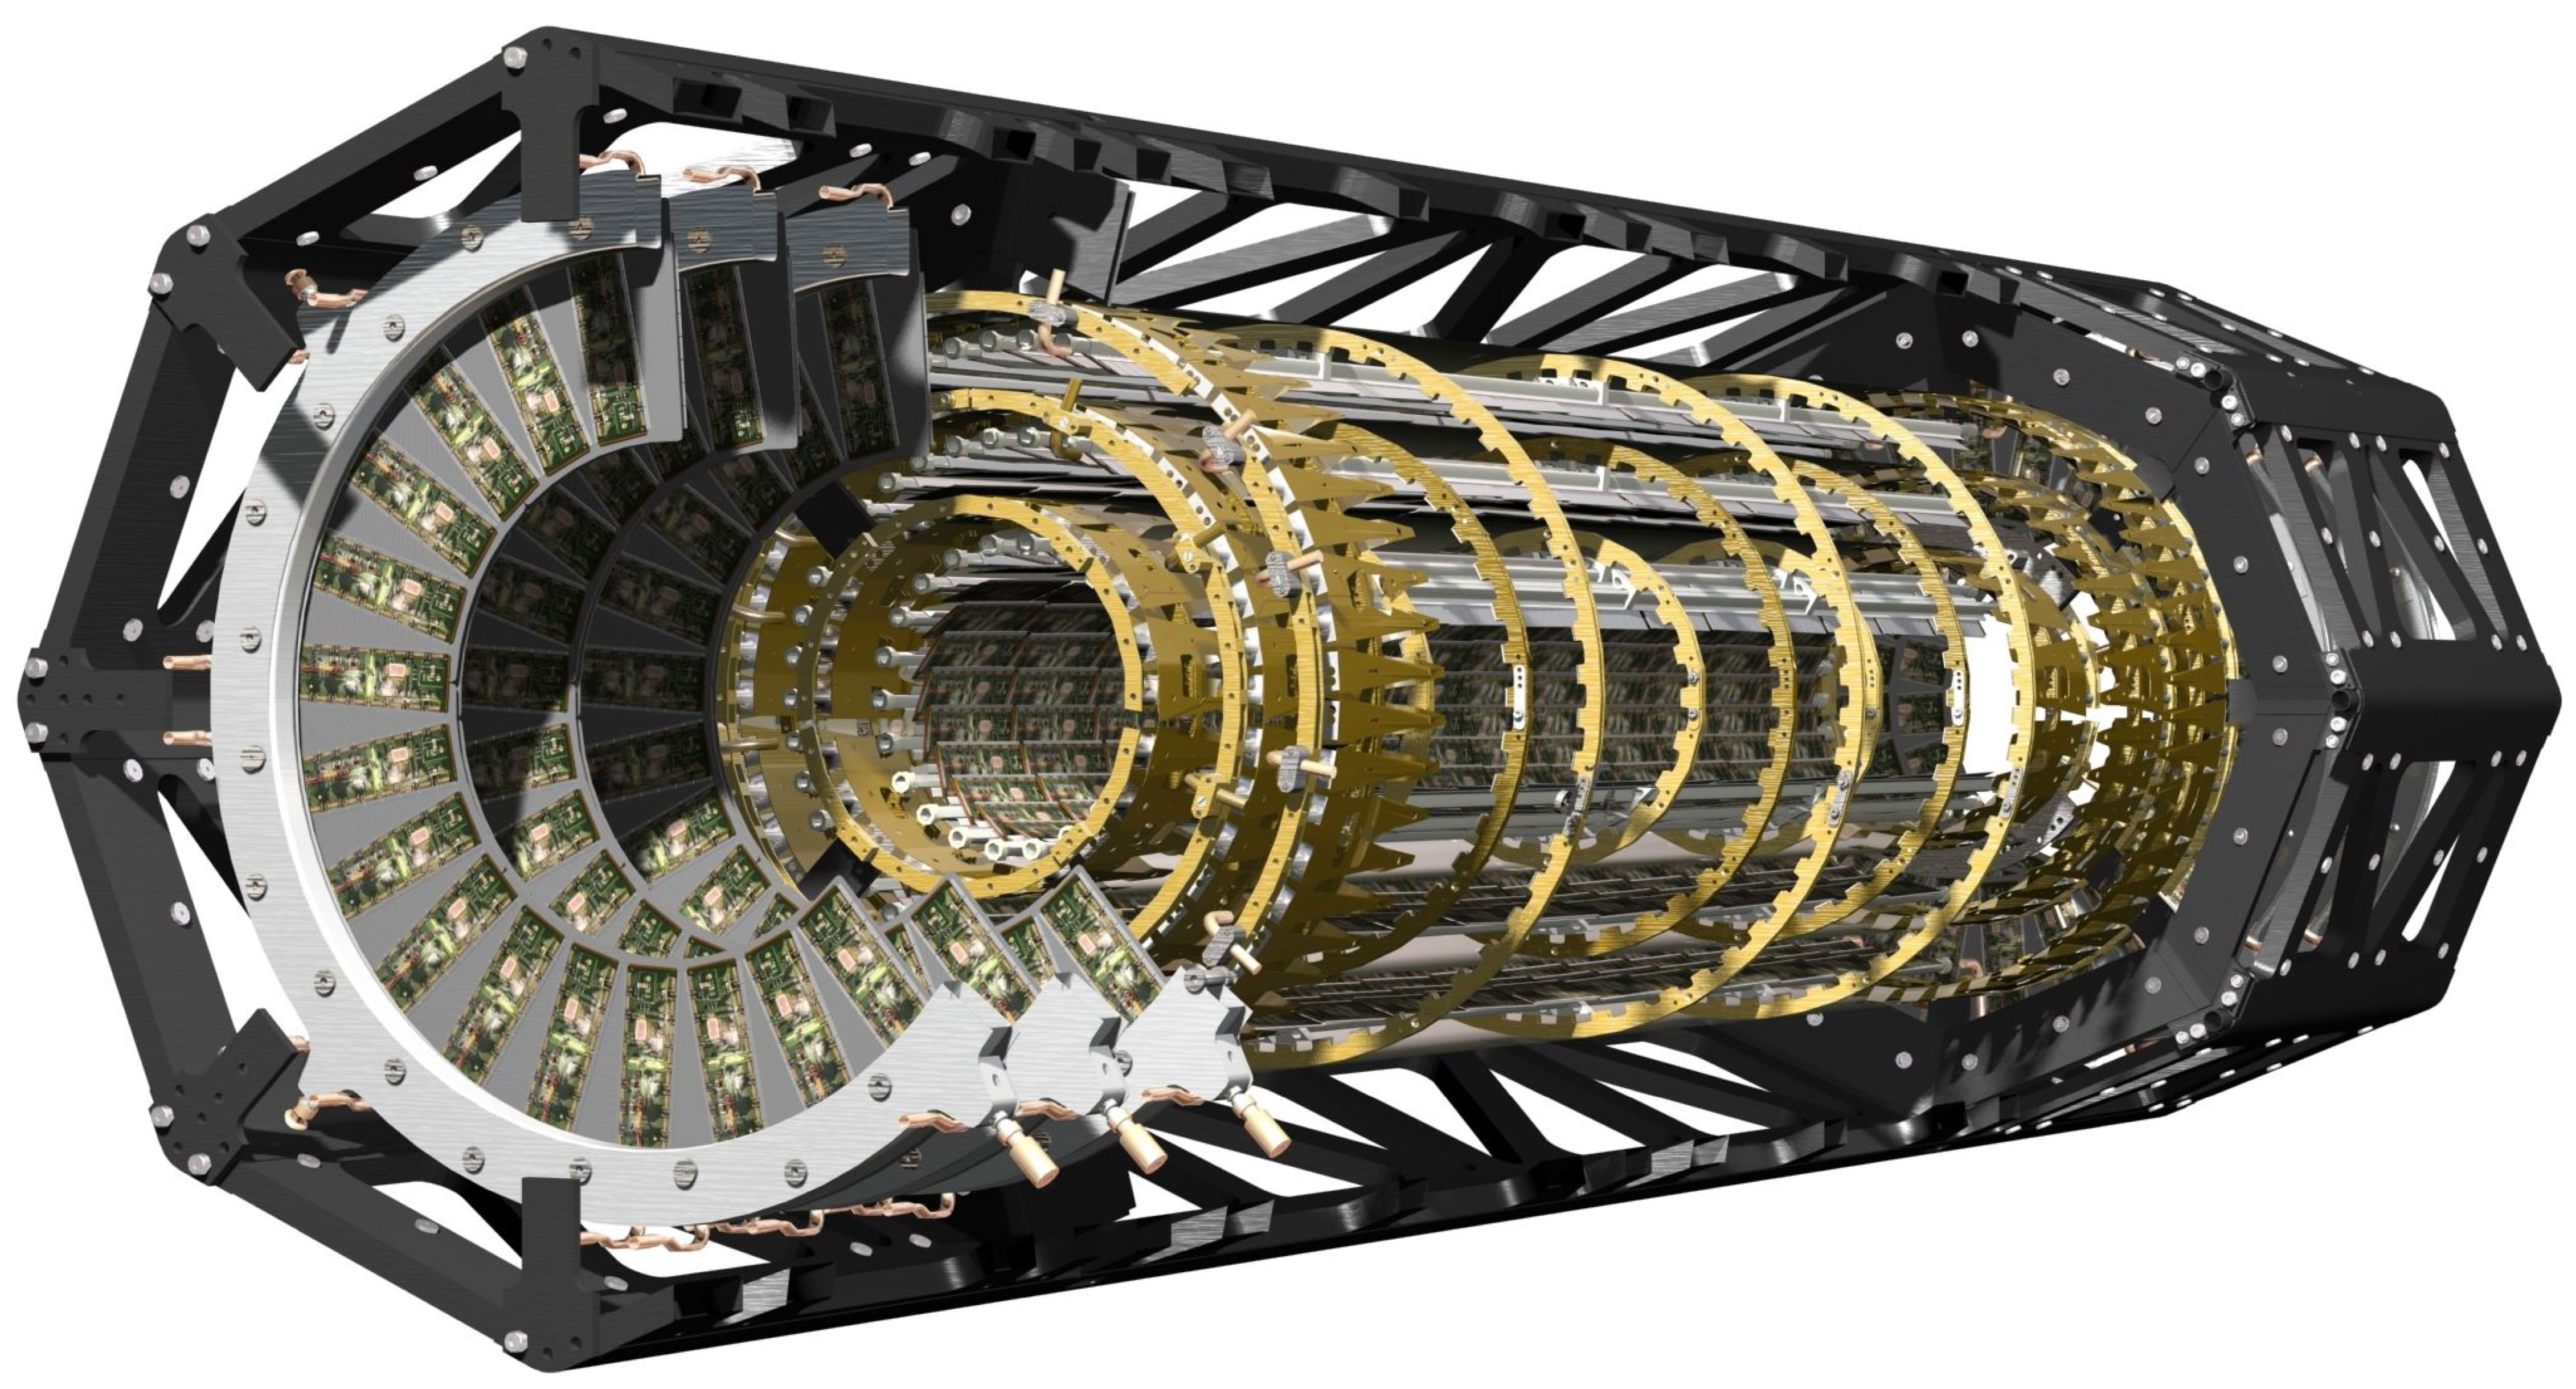
\includegraphics[width=0.6\textwidth]{ATLAS/ATLAS_pixel.eps}
 \caption[Cut-away view of the ATLAS pixel detector in the inner detector.]{%
  Cut-away view of the ATLAS pixel detector in the inner detector~\cite{Pequenao:1095925}.
  The pixel sensors form three cylindrical layers in the barrel and three consecutive disks at each end-cap.}\label{fig:ATLAS_pixel}
\end{figure}

The \Gls{SCT} surrounds the pixel detector in the barrel with four layers of stereo strips with small angle coverage $(40~\mathrm{mrad})$, shown in \Cref{fig:ATLAS_inner_detector_radial_view}, to measure hits in the silicon in both $R\textrm{-}\phi$ and $z$.
In the end-cap region, the SCT strips run radially in nine disks in each end-cap (for 18 disk in total).
In total, the SCT has roughly 6.3 million readout channels and results in track resolutions of $17~\mu\mathrm{m}~(R\textrm{-}\phi) \times 580~\mu\mathrm{m}~(z)$ in the barrel region and $17~\mu\mathrm{m}~(R\textrm{-}\phi) \times 580~\mu\mathrm{m}~(R)$ in the end-cap region.

The \Gls{TRT} further extends the ID $R\textrm{-}\phi$ information up to $\abs{\eta} = 2.0$ by providing a large number of track interactions with its approximately $351,000$ $4~\textrm{mm}$ straw tubes.
In the barrel region, the TRT straw tubes are parallel to the beam axis, shown in \Cref{fig:ATLAS_inner_detector_radial_view}, and extend for $144~\mathrm{cm}$ on either side of $\eta = 0$.
In the end-cap region, $37~\mathrm{cm}$ TRT straws are radially arranged with respect to the beamline in wheels, shown in \Cref{fig:ATLAS_inner_detector}.
Combined with the precision tracking from the pixel detectors and SCT, the tracking information that the TRT gives at larger radii contributes to high precision tracking of charged particles in both $R\textrm{-}\phi$ and $z$, and the large number of hits in the TRT significantly improve momentum measurements.

\begin{figure}[htbp]
 \centering
 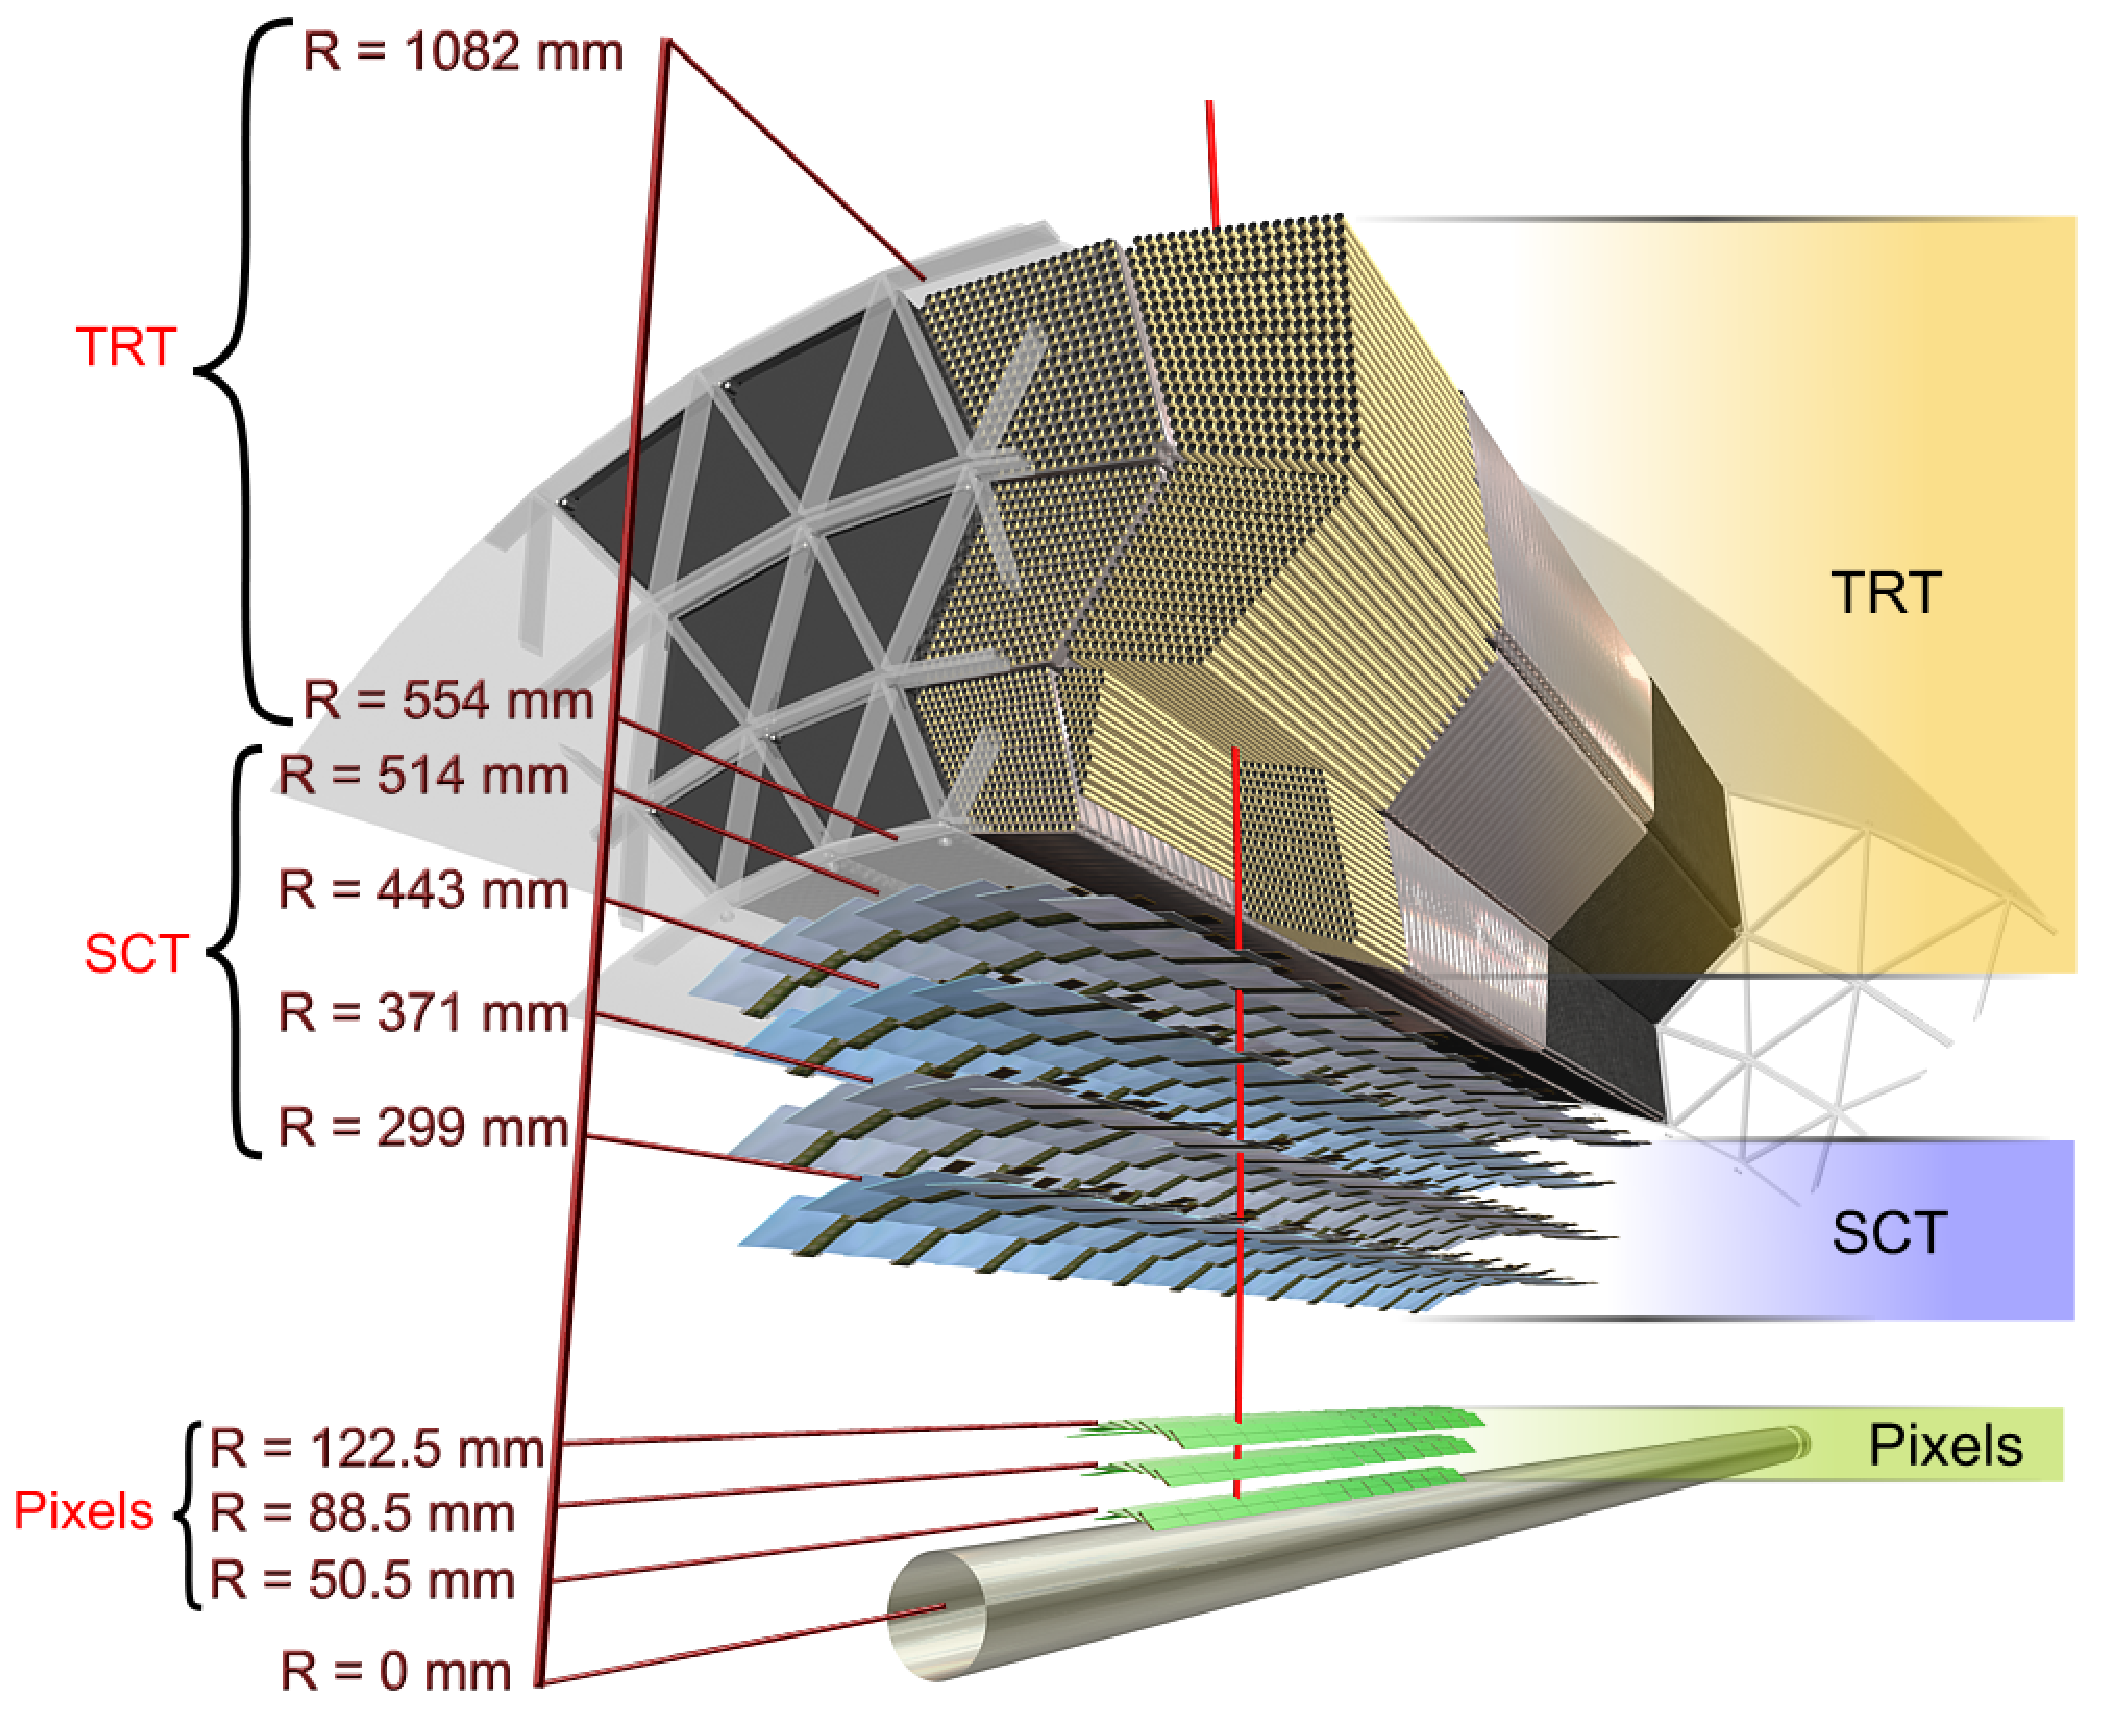
\includegraphics[width=0.6\textwidth]{ATLAS/ATLAS_inner_detector_radial_view.eps}
 \caption[Scale cut-away view of the pixel detector, Semiconductor Tracker, and Transition Radiation Tracker in the barrel-region.]{%
  The sensors and structural elements traversed by a charged track of $10~\GeV$ $p_{T}$ in the barrel inner detector $(\abs{\eta} = 0.3)$.
  The track traverses successively the beryllium beam-pipe, the three cylindrical silicon-pixel layers with individual sensor elements of $50 \times 400~\mu\mathrm{m}^{2}$, the four cylindrical double layers (one axial and one with a stereo angle of $40~\mathrm{mrad}$) of barrel SCT sensors of pitch $80~\mu\mathrm{m}$, and approximately 36 axial straws of $4~\mathrm{mm}$ diameter contained in the barrel TRT modules within their support structure~\cite{PERF-2007-01}.}\label{fig:ATLAS_inner_detector_radial_view}
\end{figure}

\section{Calorimeter System}\label{sec:ATLAS_calo}

The ATLAS calorimeter system, shown in \Cref{fig:ATLAS_calorimeter}, provides excellent energy deposition measurements for particles with coverage up to $\abs{\eta} < 4.9$ with different calorimetry subsystems for various physics processes.
In the pseudorapidity range of the inner detector ($\abs{\eta} < 2.5$) the high granularity electromagnetic (EM) liquid argon calorimeter system provides measurement of electrons and photons.
The more coarse resolution of the hadronic calorimeter systems provides measurements for jet reconstruction and missing transverse momentum, $\MET$, in conjunction with the large pseudorapidity coverage.
These calorimeter designs are both ``sampling calorimeters'', where the ``active'' materials that provide the signals are different from the ``absorber'' materials that reduce the particle energy and cause showering.
The calorimeter subsystems are also designed to be sufficiently thick as to contain the electromagnetic and hadronic showers that originate inside them, and to limit punch-through to the muon systems.

\begin{figure}[htbp]
 \centering
 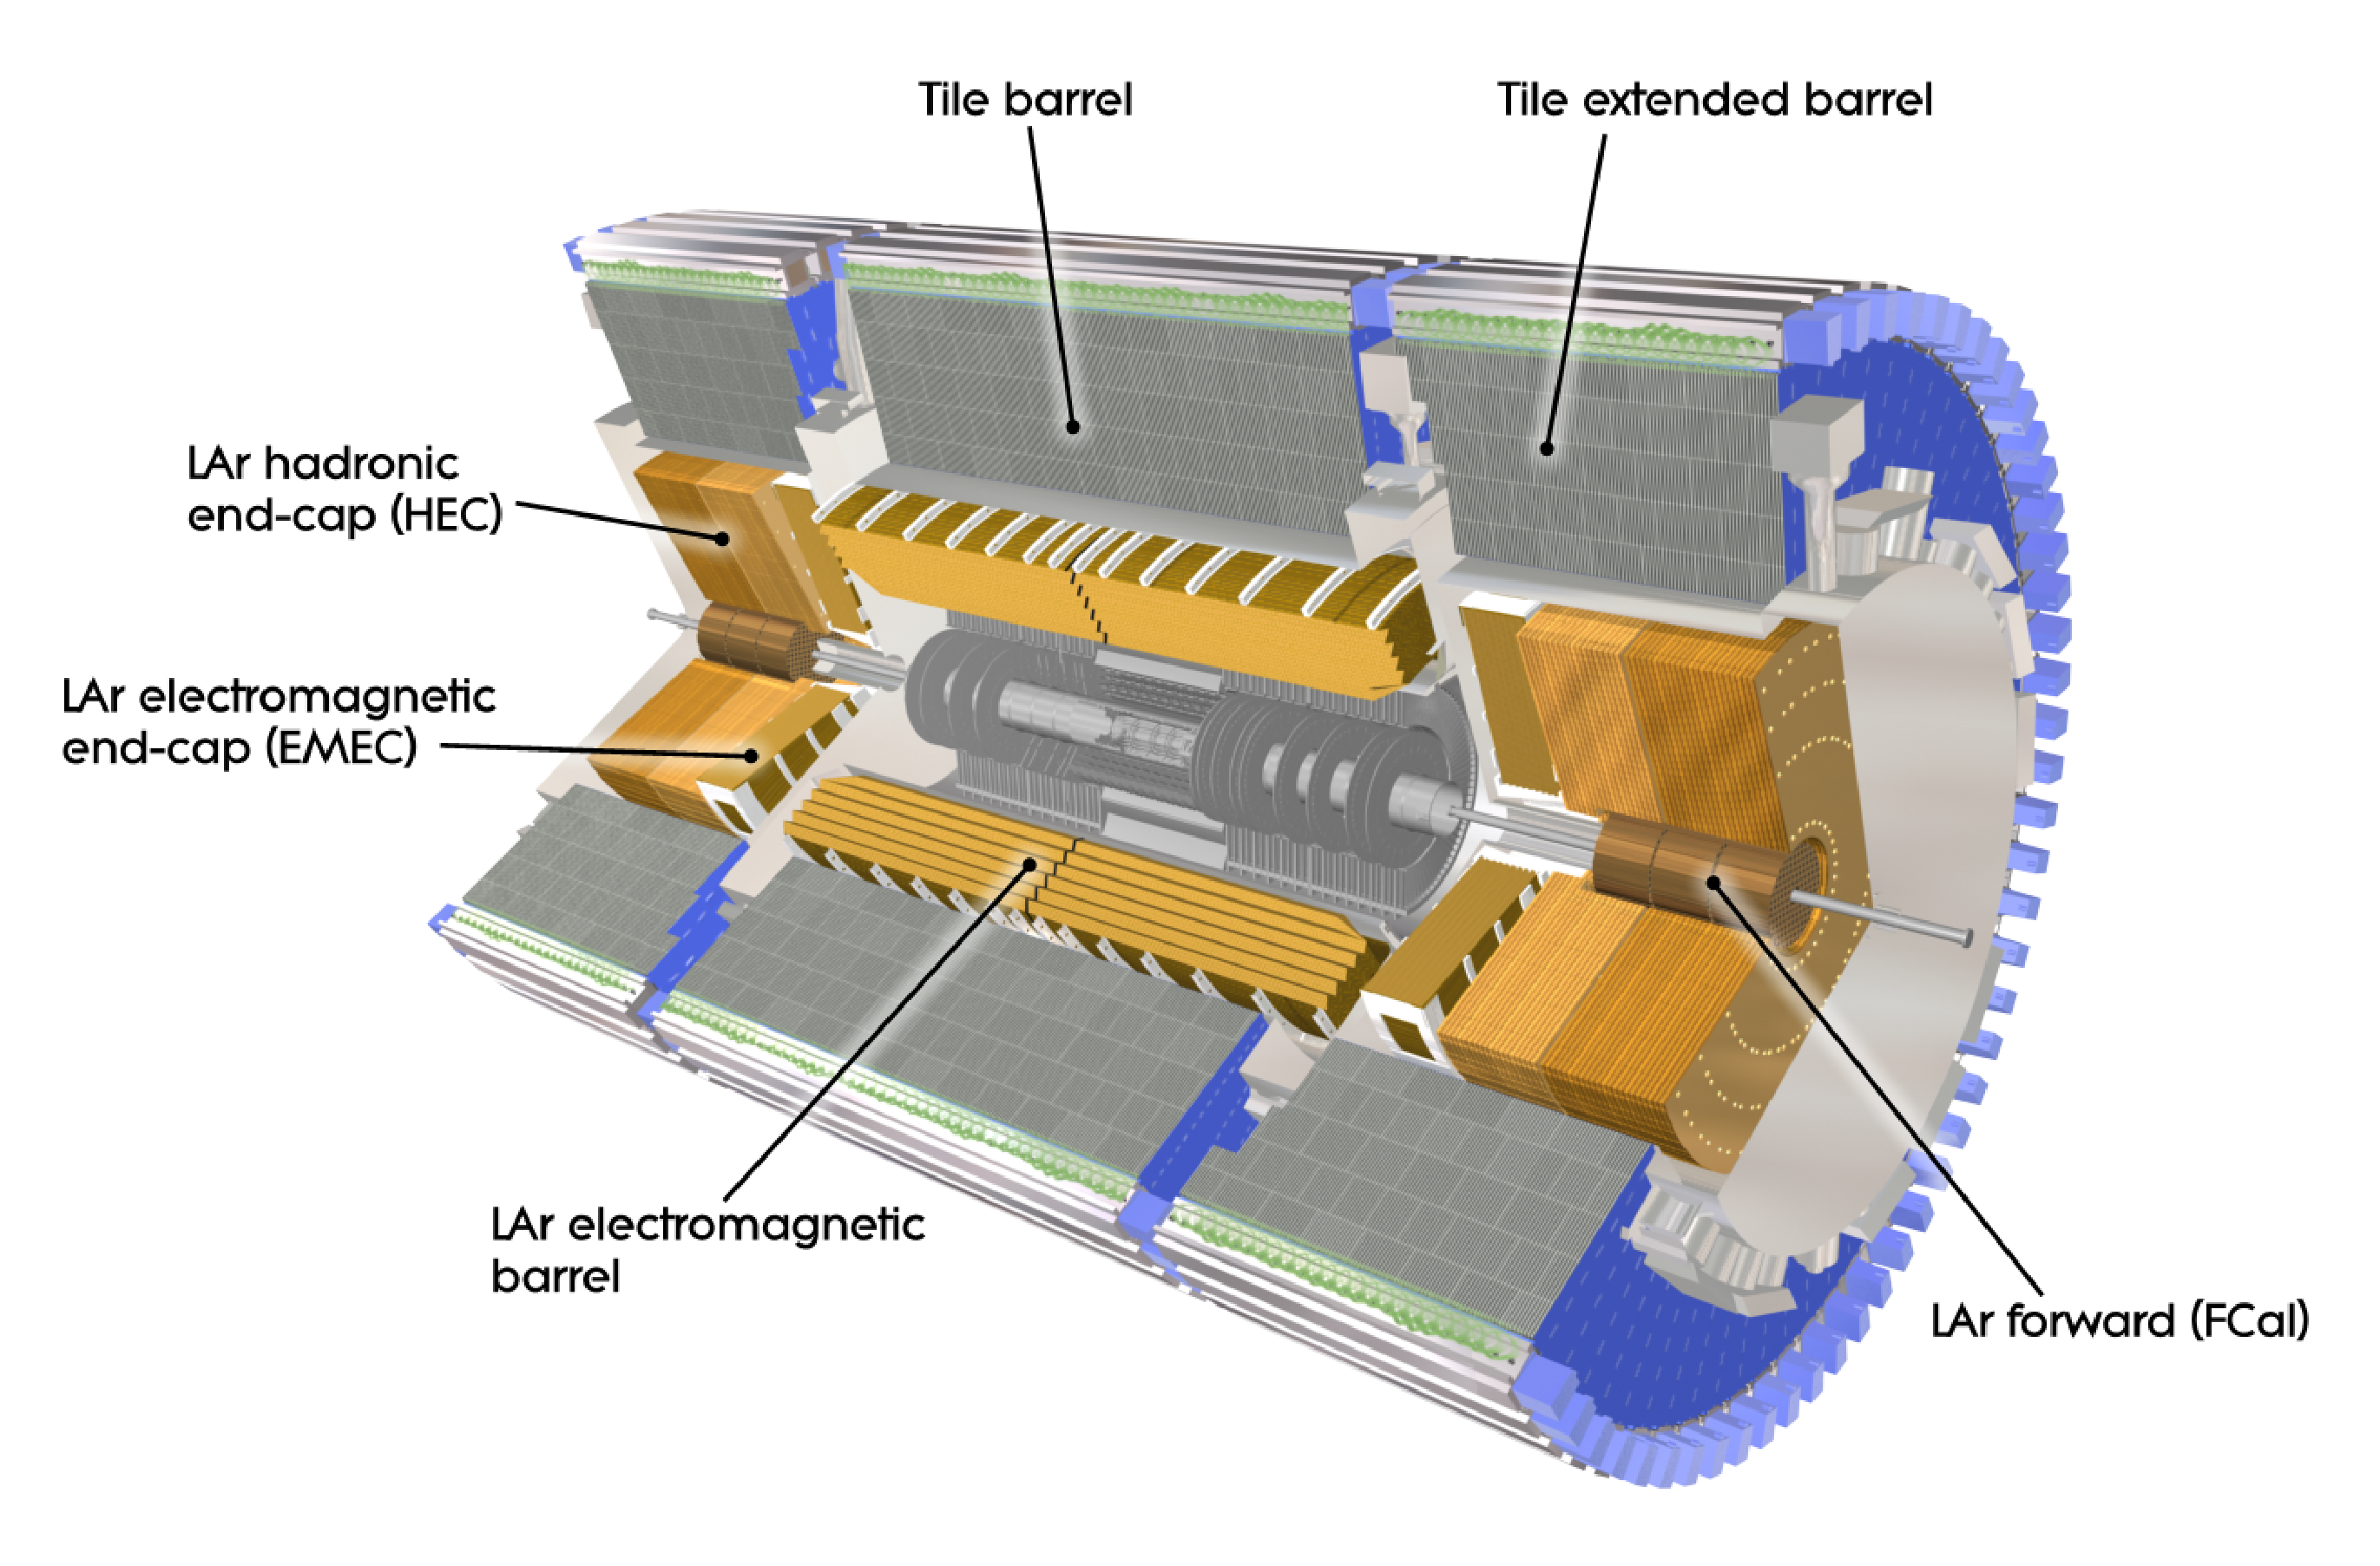
\includegraphics[width=0.7\textwidth]{ATLAS/ATLAS_calorimeter.eps}
 \caption[Cut-away view of the ATLAS calorimeter system.]{%
  Cut-away view of the ATLAS calorimeter system~\cite{Pequenao:1095927}.}\label{fig:ATLAS_calorimeter}
\end{figure}

\subsection{Electromagnetic Calorimeter}\label{sec:ATLAS_electromagnetic_calorimeter}

The electromagnetic calorimeter system, shown in \Cref{fig:ATLAS_LAr}, consists of lead-liquid argon detectors with a characteristically unique ``accordion'' lead absorber plate design that allows for continuous coverage in $\phi$ with folding angles of the accordion ``waves'' that vary with the radius to keep the LAr gap constant, as shown in \Cref{fig:ATLAS_LAr_module}.
Liquid argon (LAr) is the active detector material for the EM calorimeters as it has a linear behavior, very stable response over time, and is intrinsically radiation-hard.
In the barrel region the LAr EM calorimeter is split into symmetric half-barrels, and in the end-caps the LAr EM calorimeter exists as two coaxial wheels, respectively covering the regions of $1.375 < \abs{\eta} < 2.5$ and $2.5 < \abs{\eta} < 3.2$.

\begin{figure}[htbp]
 \centering
 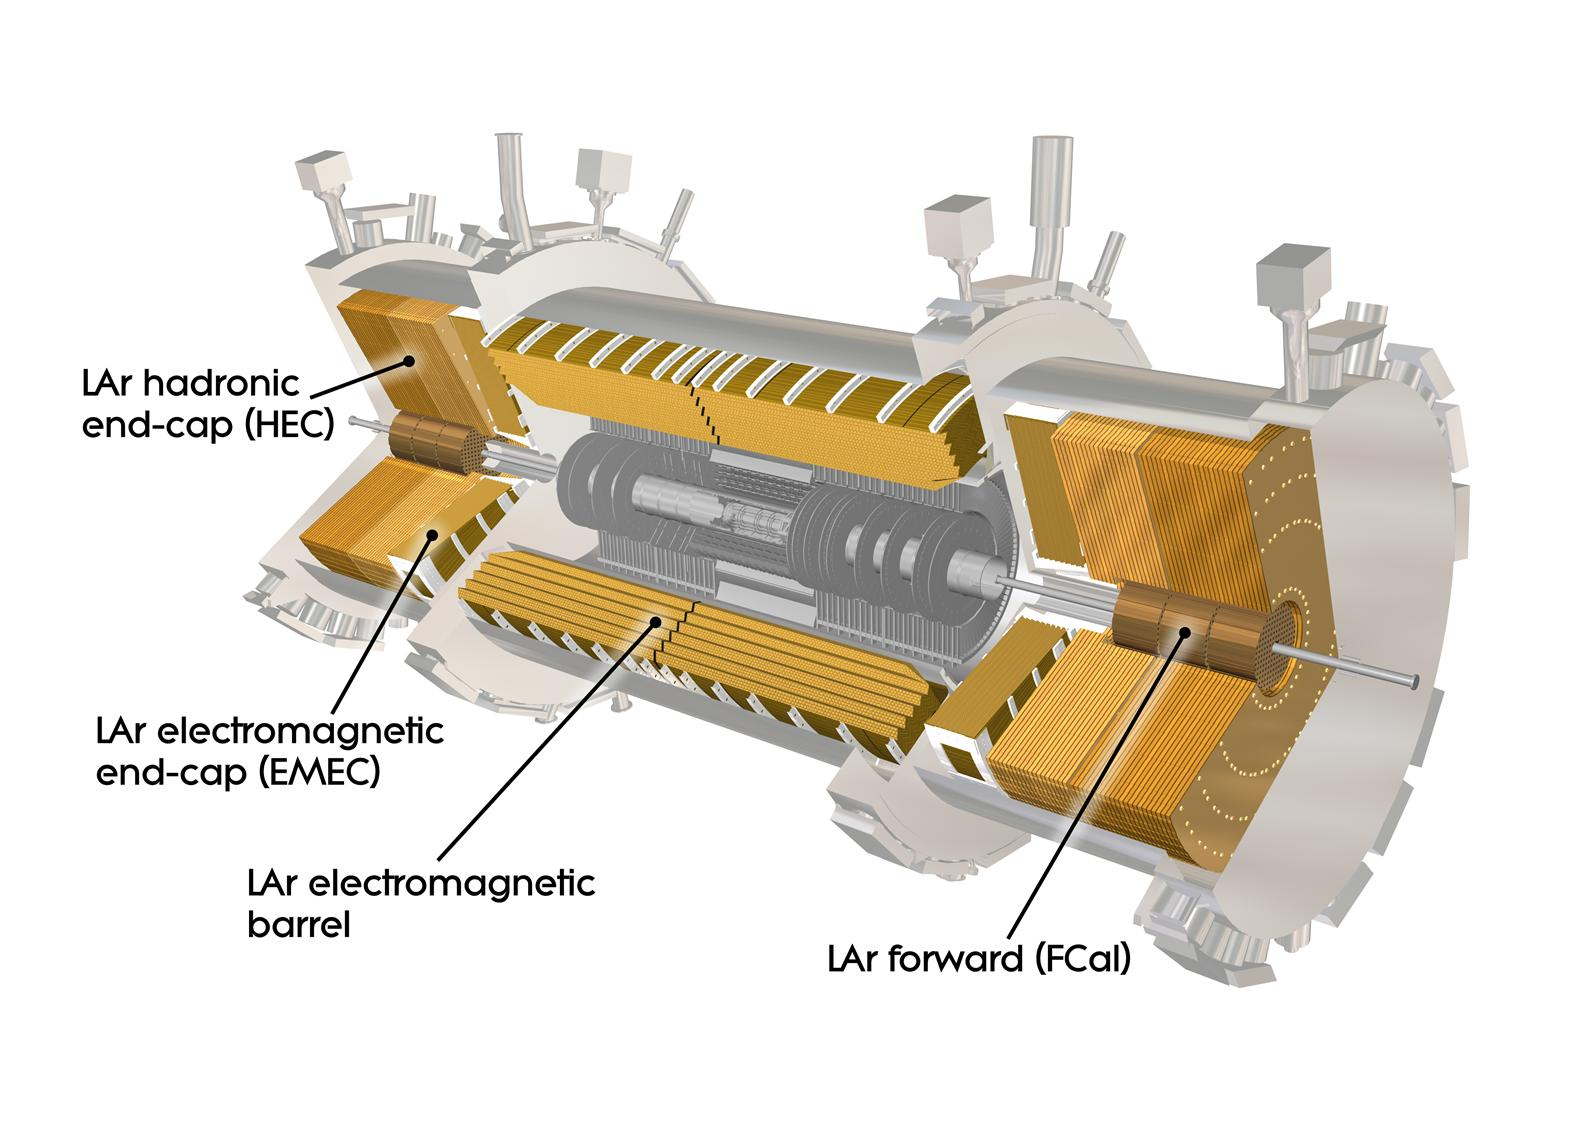
\includegraphics[width=0.7\textwidth]{ATLAS/ATLAS_LAr.jpg}
 \caption[Cut-away view of the ATLAS electromagnetic liquid argon calorimeter system.]{%
  Cut-away view of the ATLAS electromagnetic liquid argon calorimeter system~\cite{Pequenao:1095927}.}\label{fig:ATLAS_LAr}
\end{figure}

\begin{figure}[htbp]
 \centering
 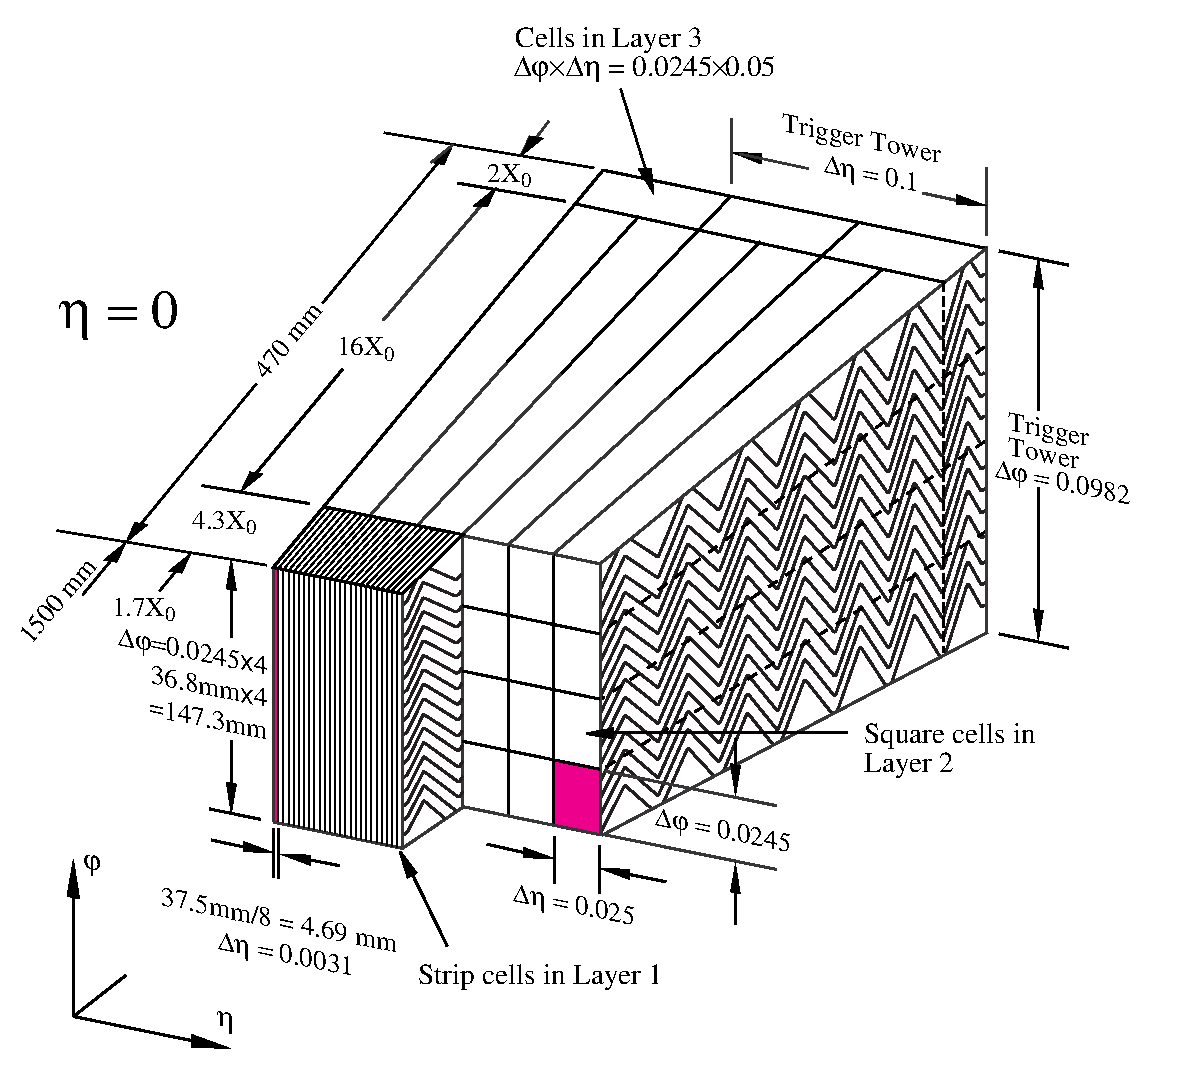
\includegraphics[width=0.6\textwidth]{ATLAS/ATLAS_LAr_module.eps}
 \caption[Sketch of a liquid argon calorimeter system barrel module detailing granularity in $\eta$ and $\phi$.]{%
  Sketch of a barrel module where the different layers are clearly visible with the ganging of electrodes in $\phi$.
  The granularity in $\eta$ and $\phi$ of the cells of each of the three layers and of the trigger towers is also shown~\cite{PERF-2007-01}.}\label{fig:ATLAS_LAr_module}
\end{figure}

\subsection{Hadronic Calorimeter}\label{sec:ATLAS_hadronic_calorimeter}

The hadronic calorimeter system is composed of the tile calorimeters in the barrel region, and the LAr Hadronic End-cap Calorimeter (HEC) and LAr Forward Calorimeter (FCal) in the end-cap region.
The tile sampling calorimeter resides outside the EM calorimeter system and provides coverage out to $\abs{\eta} < 1.7$ and radial coverage from $2.28~\mathrm{m}$ out to $4.25~\mathrm{m}$.
The tile calorimeter absorber material is steel and uses scintillating tiles as the active material, which are read out using wavelength shifting fibers into photomultiplier tubes.
The HEC exists as two wheels in each end-cap behind the end-cap EM calorimeter, extending the coverage in the end-caps out to $\abs{\eta} < 3.2$.
The copper absorber plates of the HEC are interleaved with $8.5~\mathrm{mm}$ spacers of LAr providing active material.
The FCal extends coverage from $3.1 < \abs{\eta} < 4.9$ and is composed of three modules in each end-cap: a copper module optimized for electromagnetic measurements, and then two made of tungsten for hadronic interaction measurements.
The modules are a metal matrix with regularly spaced longitudinal channels consisting of tubes with a concentric rod and LAr filling the gap between them.

For calorimetry systems the energy resolution improves as the energy of the particle, $E$ increases, generally as $1/\sqrt{E}$.
More specifically, the energy resolution, $\sigma\left(E\right)$, of a calorimeter is given as the quadrature sum%
\footnote{That is, $a \oplus b = \sqrt{a^{2} + b^{2}}$.}
\begin{equation}
 \frac{\sigma\left(E\right)}{E} = \frac{a}{\sqrt{E}} \oplus \frac{b}{E} \oplus c\,,
 \label{eq:calorimeter_energy_resolution}
\end{equation}
where $a$ is the ``stochastic term'' for intrinsic shower fluctuations, $b$ is the ``noise term'', and $c$ is the ``constant'' term~\cite{Fabjan:692252}.
It is seen from \Cref{eq:calorimeter_energy_resolution} that at lower energies the stochastic term is more important and at higher energies the constant term affects the energy resolution more.
The ATLAS calorimeters are designed to have excellent energy resolution, which is clearly seen from the observed energy resolution for the ATLAS LAr EM calorimeter barrel region in testbeam experiments~\cite{Ilic:2014,Aleksa:1547314}
\[
 \frac{\sigma\left(E\right)}{E} = \frac{10\%}{\sqrt{E}} \oplus \frac{200~\MeV}{E} \oplus 0.2\%\,.
\]
For the hadronic calorimeters the stochastic term is required to be under $50\%$ and the constant term under $3\%$~\cite{Ilic:2014}.

\section{Muon Spectrometer}\label{sec:ATLAS_muon_spectrometer}

The ATLAS \gls{muon spectrometer}, shown in \Cref{fig:ATLAS_muon_spectrometer}, is arranged as the exterior detector subsystem to provide coverage for muons deflected from the air-core toroid magnets.
As muons are minimum ionizing particles%
\footnote{The mass stopping power for muons in the typical energy ranges at the LHC is less than $4~\MeV\,\mathrm{cm}^{2}/\mathrm{g}$.
 To put this in context, a $1~\GeV$ muon can punch through roughly $1~\mathrm{m}$ of iron before stopping~\cite{Garutti:lecture}.}
, as seen in \Cref{fig:Bethe-Bloch_stopping_power}, they pass through the inner detector and calorimeter systems while being radially deflected by the solenoid magnetic field before entering the toroidal magnetic field and getting deflected along $\hat{\vec{z}}$.
Given the resulting trajectories, in the barrel region muon tracks are measured by three cylindrical layers of \glspl{MDT}, shown in \Cref{fig:ATLAS_MDT_chamber} and \Cref{fig:ATLAS_muon_barrel_track}, and in the end-caps region three planes of MDT wheels before escaping the detector altogether --- hence the name \emph{spectrometer}.
For most of the $\eta$ range the MDTs perform most of the precision measurements of the tracks, though from $2 < \abs{\eta} < 2.7$ higher granularity \glspl{CSC} provide tracking to withstand the intense rate and radiation~\cite{PERF-2007-01}.

\begin{figure}[htbp]
 \centering
 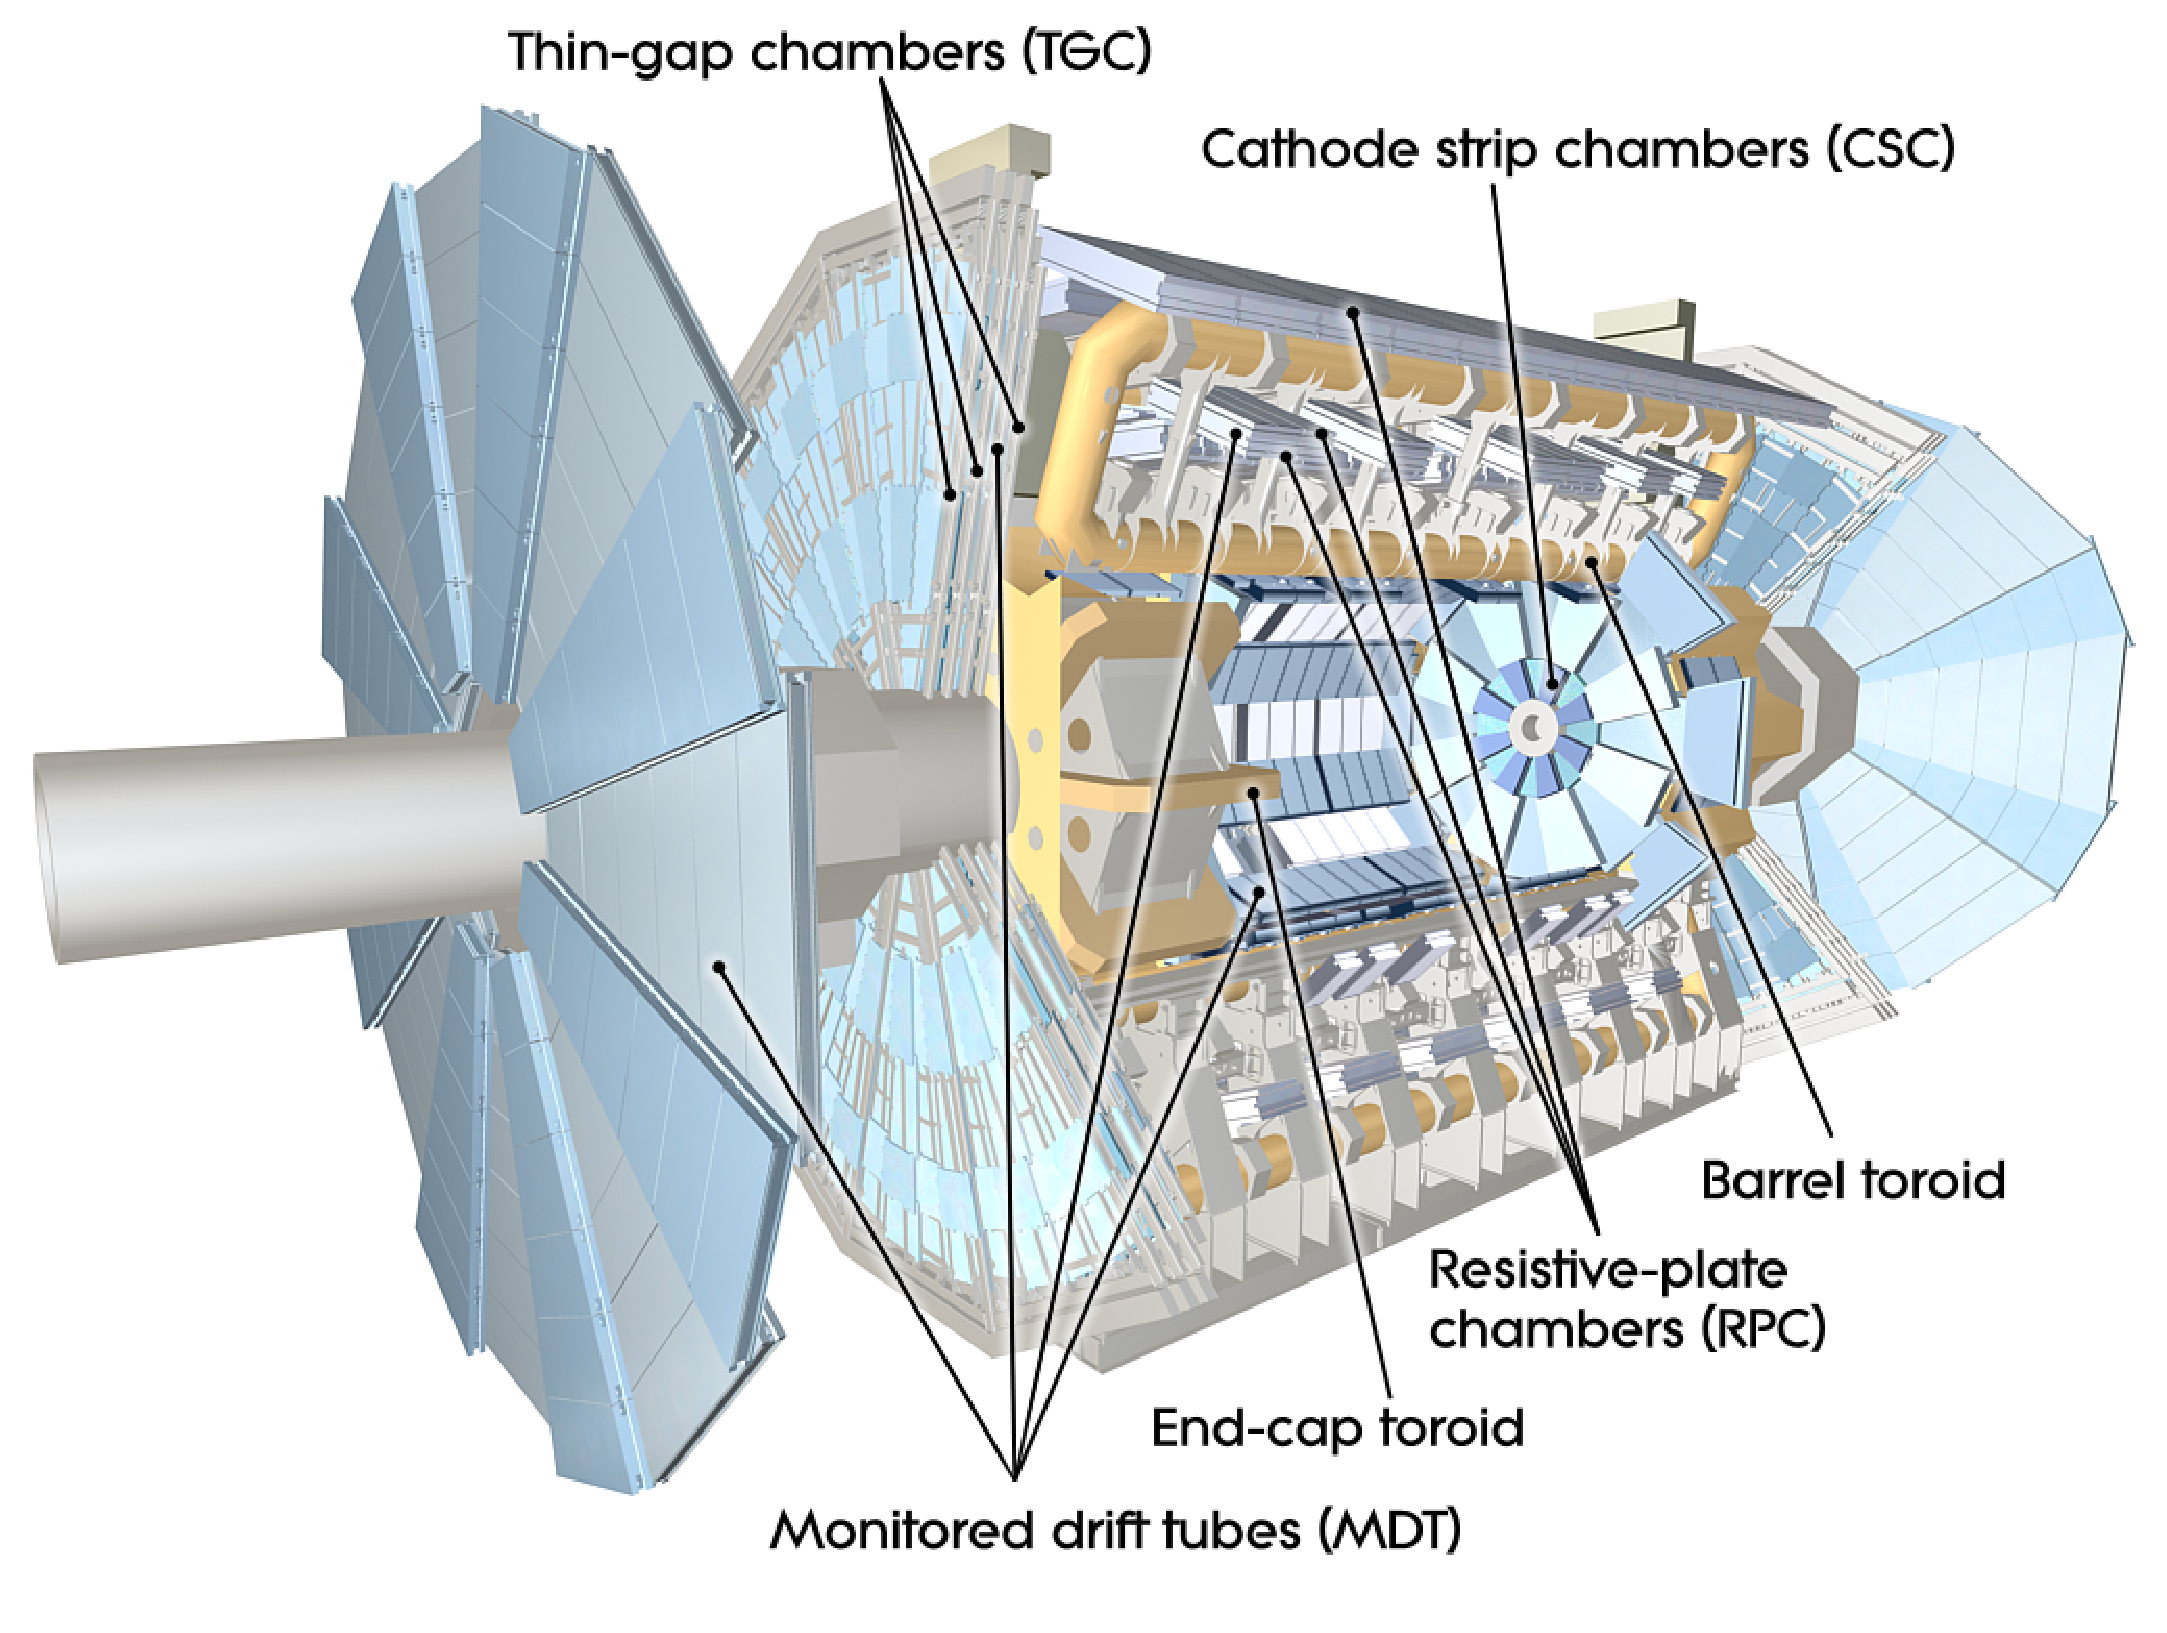
\includegraphics[width=0.6\textwidth]{ATLAS/ATLAS_muon_spectrometer.eps}
 \caption[Cut-away view of the ATLAS muon system.]{%
  Cut-away view of the ATLAS muon system~\cite{PERF-2007-01}.}\label{fig:ATLAS_muon_spectrometer}
\end{figure}

\begin{figure}[htbp]
 \centering
 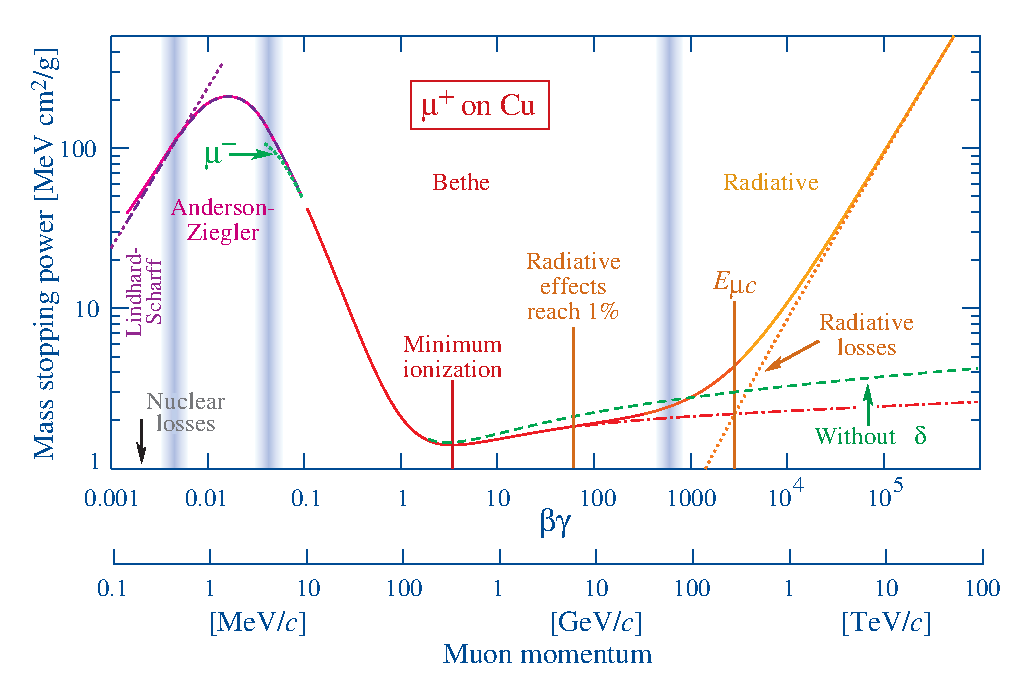
\includegraphics[width=\textwidth]{ATLAS/Bethe-Bloch_stopping_power.eps}
 \caption[Mass stopping power for positive muons in copper as a function of $\beta \gamma = p/Mc$.]{%
  Mass stopping power $\left(= \left<-dE/dx\right>\right)$ for positive muons in copper as a function of $\beta \gamma = p/Mc$ over nine orders of magnitude in momentum (12 orders of magnitude in kinetic energy).
  Solid curves indicate the total stopping power.
  Data below the break at $\beta \gamma \approx 0.1$ are taken from ICRU 49~\cite{ICRU49}, and data at higher energies are from~\cite{Groom:2001kq}.
  Vertical bands indicate boundaries between different approximations discussed in~\cite{PDG2018:Ch33}.
  The short dotted lines labeled ``$\mu^{-}$'' illustrate the ``Barkas effect'', the dependence of stopping power on projectile charge at very low energies~\cite{PhysRev.101.778}.
  $dE/dx$ in the radiative region is not simply a function of $\beta$~\cite{PDG2018:Ch33}.}\label{fig:Bethe-Bloch_stopping_power}
\end{figure}

\begin{figure}[htbp]
 \centering
 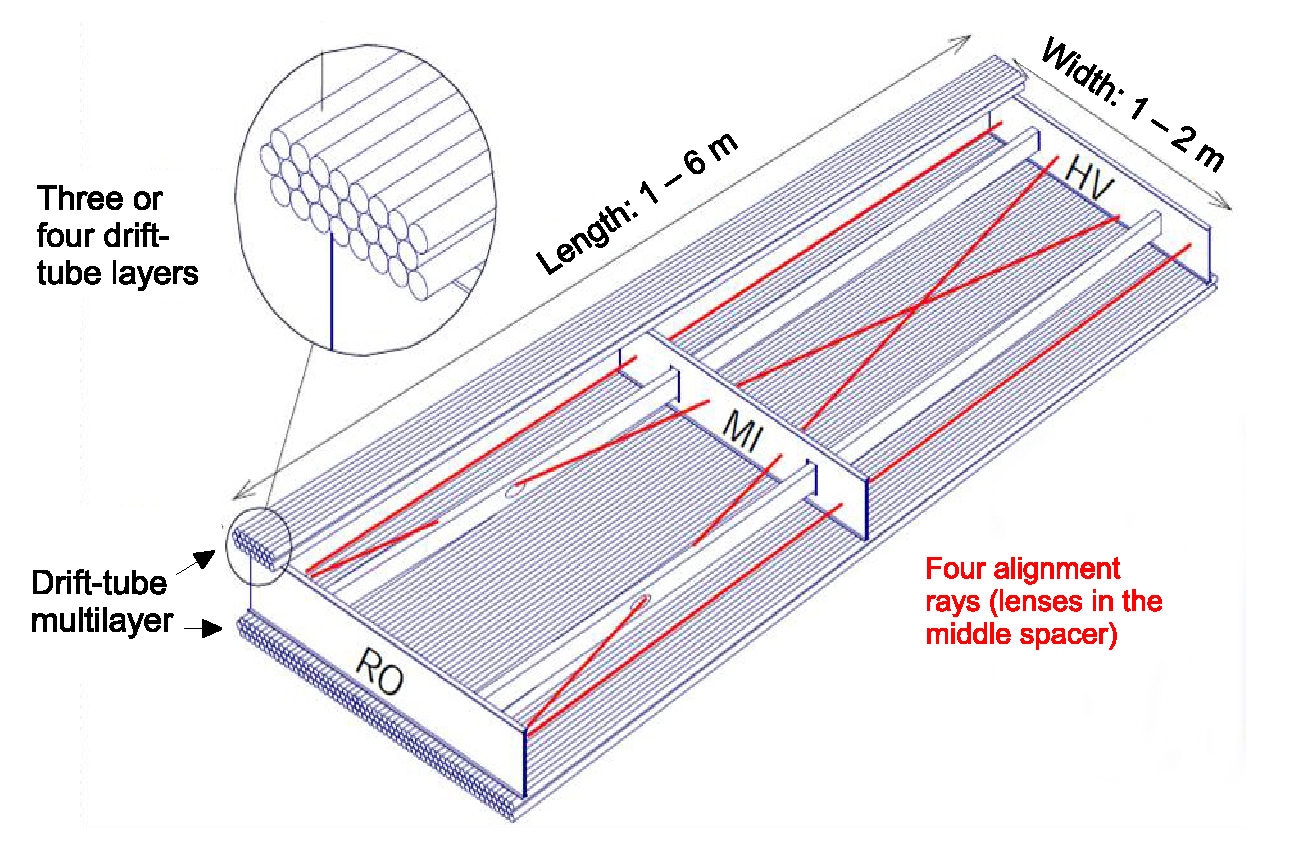
\includegraphics[width=0.6\textwidth]{ATLAS/ATLAS_MDT_chamber.eps}
 \caption[Mechanical structure of a \acrlong{MDT} chamber.]{%
  Mechanical structure of a \gls{MDT} chamber.
  Three spacer bars connected by longitudinal beams form an aluminium space frame, carrying two multi-layers of three or four drift tube layers.
  Four optical alignment rays, two parallel and two diagonal, allow for monitoring of the internal geometry of the chamber.
  RO and HV designate the location of the readout electronics and high voltage supplies, respectively~\cite{PERF-2007-01}.}\label{fig:ATLAS_MDT_chamber}
\end{figure}

\begin{figure}[htbp]
 \centering
 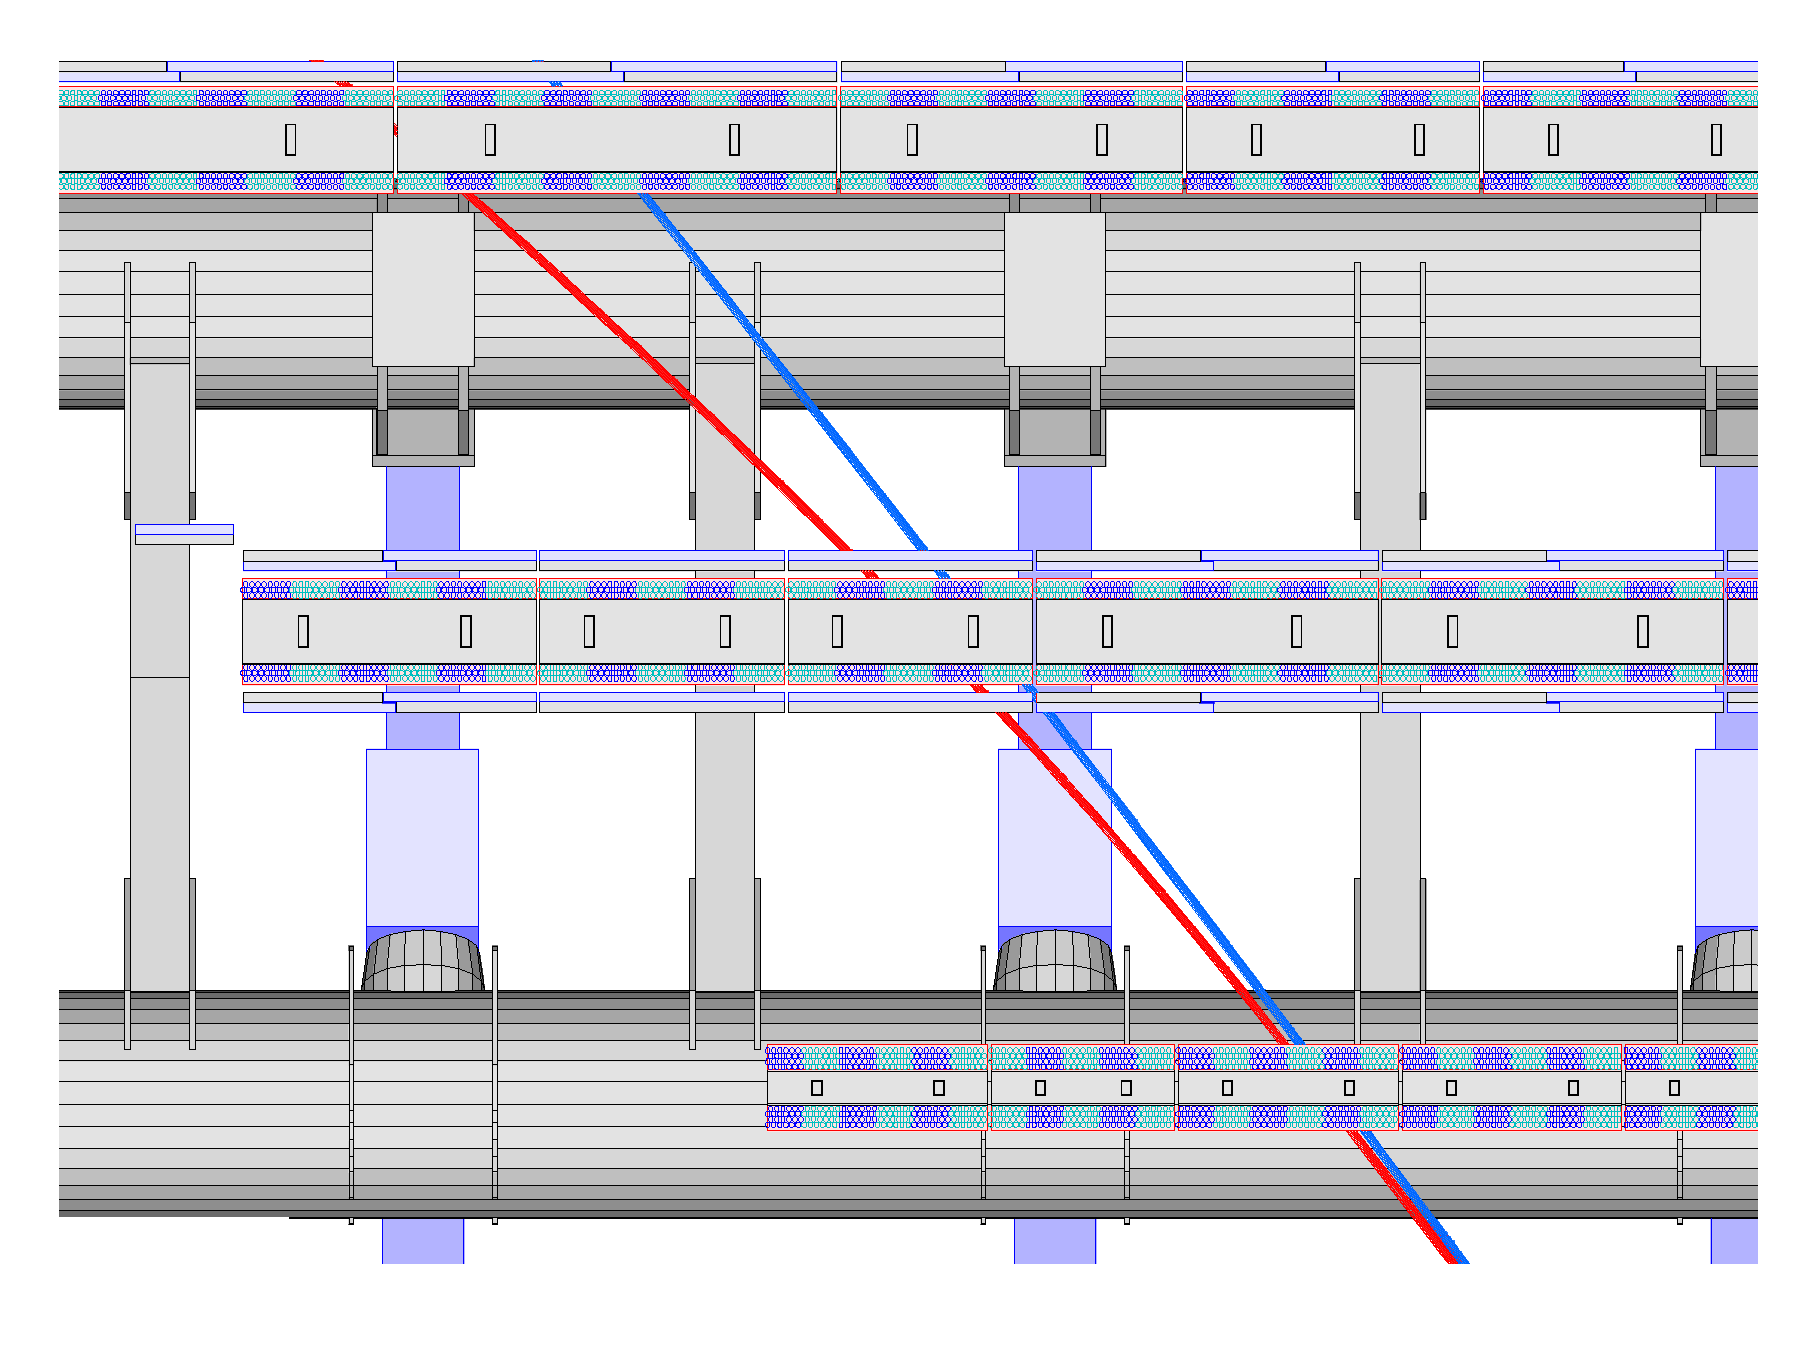
\includegraphics[width=0.6\textwidth]{ATLAS/ATLAS_muon_barrel_track.eps}
 \caption[Trajectories of muons through the three layers of \acrlong{MDT} of the barrel muon spectrometer.]{%
  Trajectories of muons with momenta of $4~\GeV$ and $20~\GeV$ in the bending plane of the barrel muon spectrometer.
  In general, the tracks cross $2 \times 4$ inner, $2 \times 3$ middle, and $2 \times 3$ outer layers of \gls{MDT} tubes.
  The cyan and dark blue areas in each MDT layer illustrate the granularity of the mezzanine cards~\cite{PERF-2007-01}.}\label{fig:ATLAS_muon_barrel_track}
\end{figure}

The trigger system for the muon system provides coverage out to $\abs{\eta} < 2.4$ and the \gls{RPC} and \gls{TGC} trigger chambers uniquely provide bunch-crossing identification, well-defined $p_{T}$ thresholds, and measurements of the muon track coordinate in the orthogonal direction of the precision-tracking chambers~\cite{PERF-2007-01}.

\section{Trigger and Data Acquisition}\label{sec:ATLAS_TDAQ}

The ATLAS \gls{TDAQ} systems, shown in \Cref{fig:ATLAS_TDAQ_system}, function collectively at two different levels: the L1 trigger and the \gls{HLT}.
Collectively, the trigger system is responsible for reducing the $40~\mathrm{MHz}$ event rate from the $25~\mathrm{ns}$ bunch crossings --- which is not possible to write out and save in real time --- to a much more manageable $1~\mathrm{kHz}$ that can be written to storage~\cite{TRIG-2016-01}.
With raw event sizes of approximately $1.6~\mathrm{Mbytes}$ this still results in data generation of over a Gigabyte per second.

\begin{figure}[htbp]
 \centering
 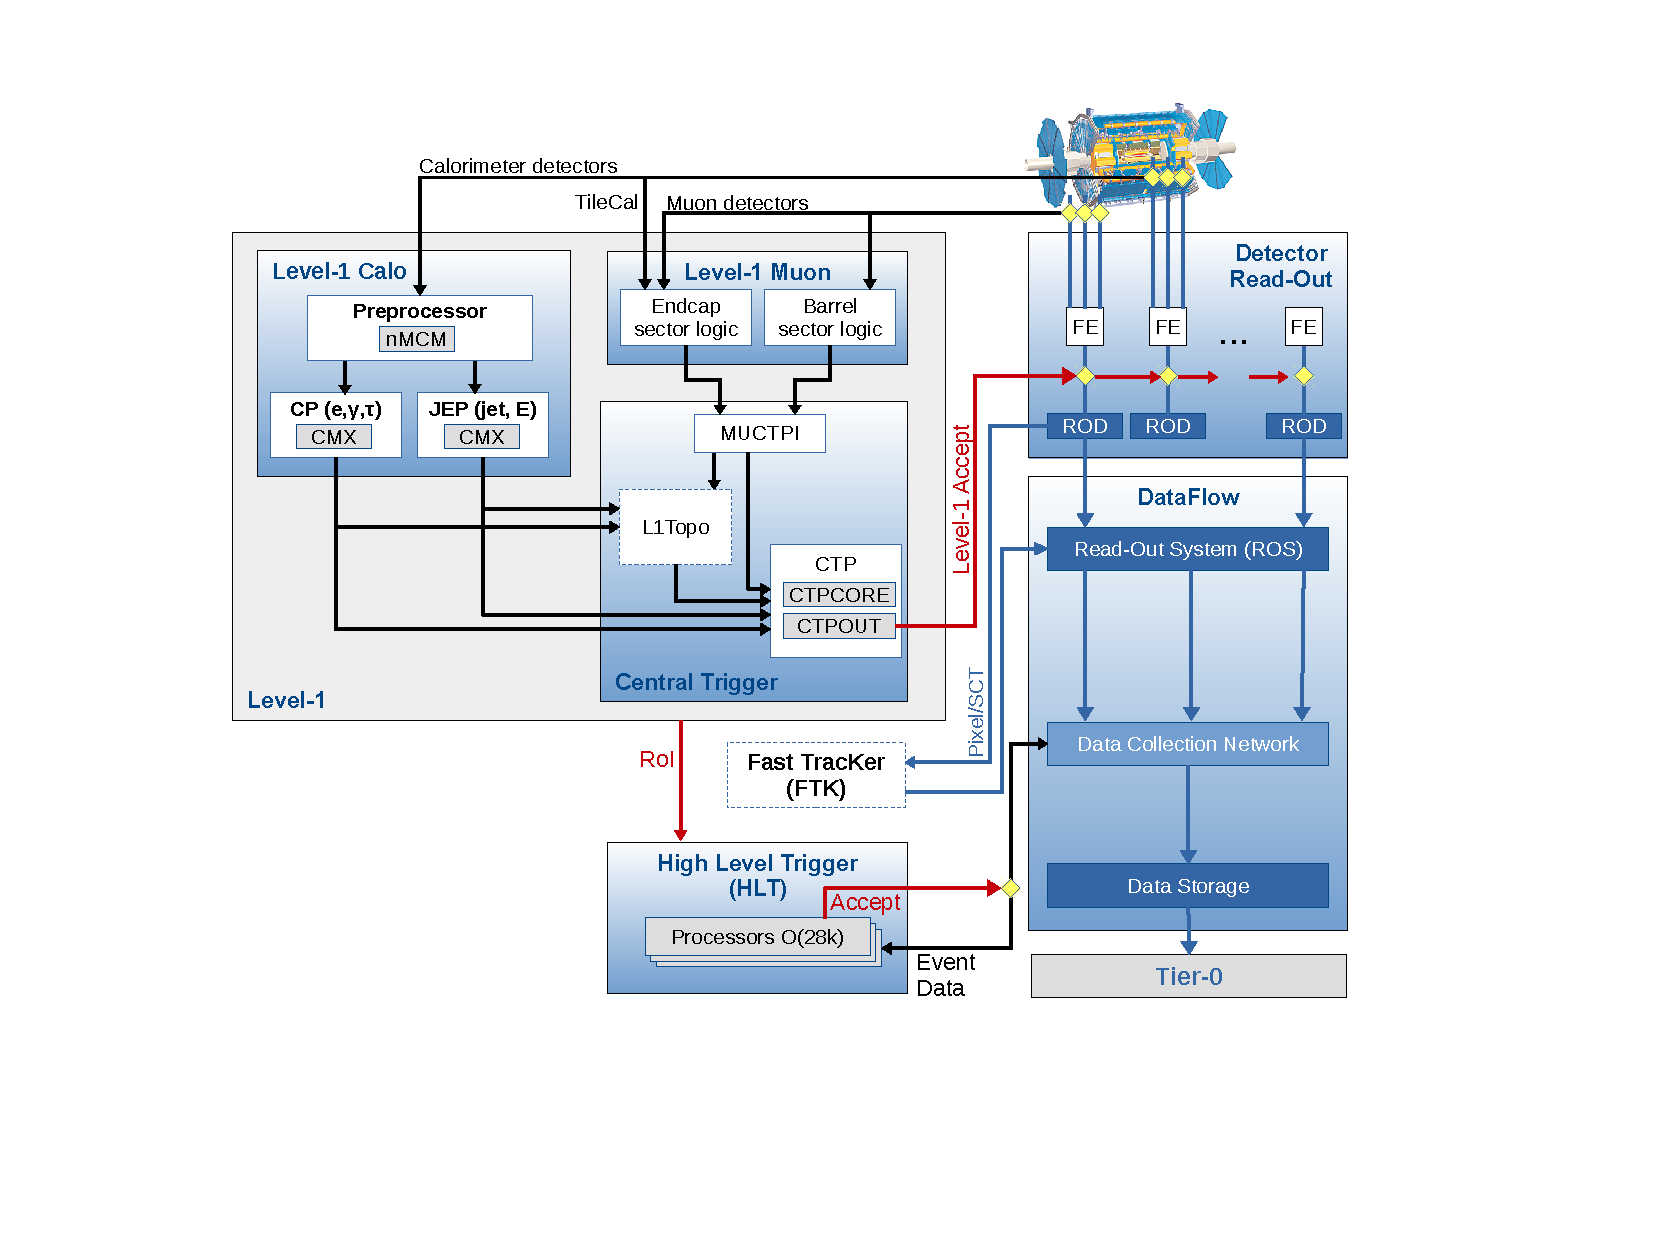
\includegraphics[width=\textwidth]{ATLAS/ATLAS_TDAQ_system.pdf}
 \caption[The ATLAS \acrlong{TDAQ} system in Run 2 with emphasis on the components relevant for triggering.]{%
  The ATLAS \gls{TDAQ} system in Run 2 with emphasis on the components relevant for triggering.
  L1Topo was installed in 2016 and commissioned during Run 2 and FTK is an upgrade for Run 3~\cite{TRIG-2016-01}.}\label{fig:ATLAS_TDAQ_system}
\end{figure}

\subsection{Level-1 Trigger (L1)}\label{sec:ATLAS_L1_trigger}

The Level-1 trigger (L1) is a hardware trigger system responsible for taking data coming from the ATLAS calorimeter and muon systems and identifying \gls{RoI}, shown in \Cref{fig:ATLAS_L1Calo_trigger_tower}, for cluster trigger candidates and further decision making within $2.5~\mu\mathrm{s}$ after the bunch-crossing associated with the event~\cite{PERF-2007-01}.
The L1Calo trigger algorithms search for high transverse momentum electrons, photons, jets, hadronically decaying $\tau$-leptons, and large $\MET$ signatures.
It does this by identifying RoIs in a sliding $4 \times 4$ window of trigger tower clusters in the calorimeters and using information from six elements formed from the sum of transverse energy in trigger tower groups~\cite{Eisenhandler:792528}:
\begin{enumerate}
 \item Four trigger tower regions (the sums shown in \Cref{fig:ATLAS_L1Calo_trigger_tower}) that measure the $\ET$ of EM showers.
 \item A hadronic core (the red box in \Cref{fig:ATLAS_L1Calo_trigger_tower}) from the four hadronic towers centered behind the EM clusters whose sum is used for isolation in the hadronic calorimeter.
 \item Four hadronic clusters summed over the EM and hadronic calorimeters that measure the $\ET$ of hadronic showers.
 \item An EM isolation ring formed from the twelve EM towers surrounding the EM core whose sum is used for isolation checks in the EM calorimeter.
 \item A hadronic isolation ring formed from the twelve hadronic towers behind the EM isolation ring whose sum is used for isolation checks in the hadronic calorimeter.
 \item A $2 \times 2 $ tower cluster RoI centered in the algorithm window and summed over the EM cluster region and hadronic core used to identify candidate RoIs.
\end{enumerate}

From these six elements algorithms then make decisions on the order of nanoseconds to classify the window as containing an EM cluster trigger candidate or a hadronic cluster trigger candidate\footnote{It is worth reflecting here that given the stringent requirements that the L1 trigger must meet that the fantastically complex objects that are hadronic jets start off as a L1 trigger tower square.} to be given to the Central Trigger for L1 trigger decision making.

\begin{figure}[htbp]
 \centering
 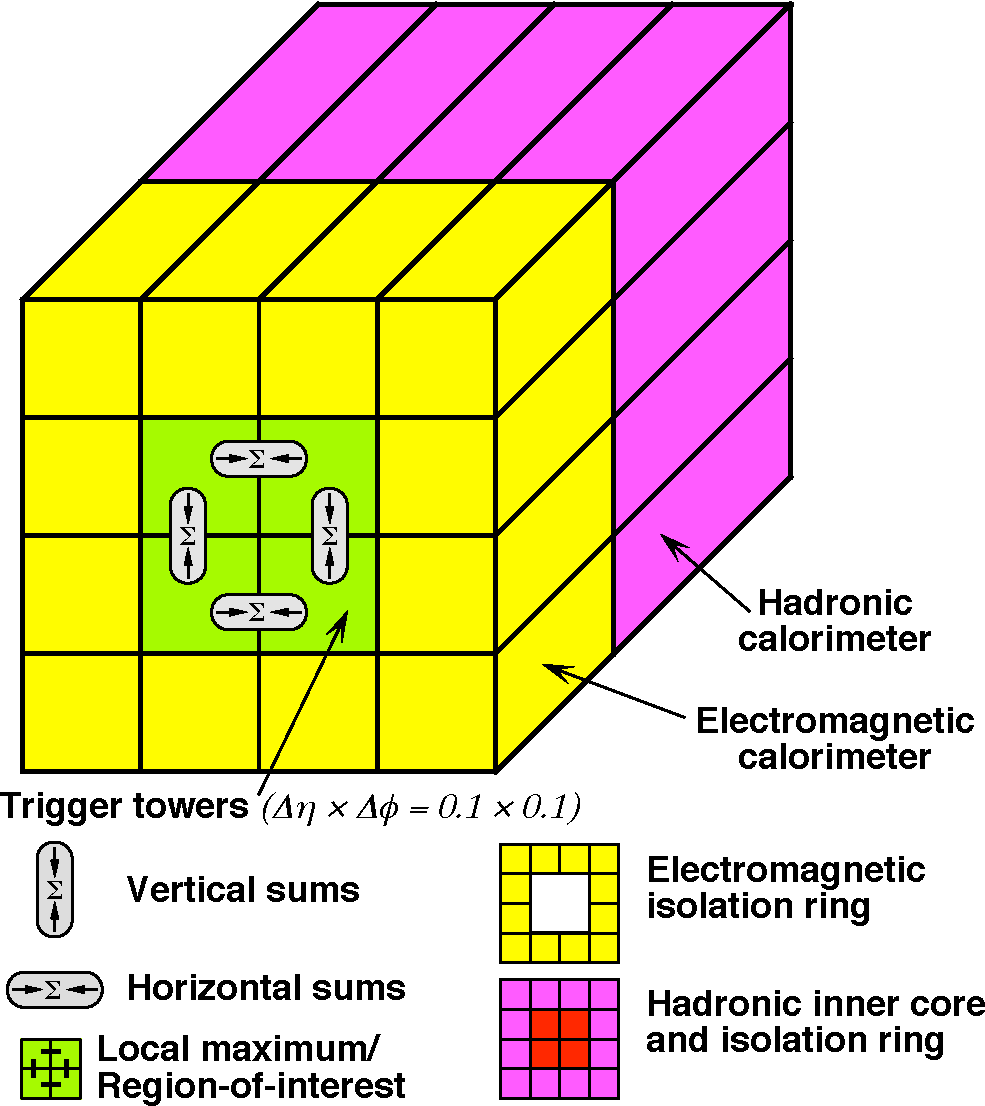
\includegraphics[width=0.4\textwidth]{ATLAS/ATLAS_L1Calo_trigger_tower.pdf}
 \caption[Schematic view of the trigger towers in a region of interest window used as input to the L1Calo trigger algorithms.]{%
  Schematic view of the trigger towers in a RoI window used as input to the L1Calo trigger algorithms~\cite{TRIG-2016-01}.}\label{fig:ATLAS_L1Calo_trigger_tower}
\end{figure}

Simultaneously in L1, the L1Muon trigger uses trigger chambers in the barrel and end-cap regions of the muon spectrometer.
Information from events with large transverse energy are then sent to the L1 topological processor (L1Topo) in the Central Trigger for a trigger decision.
The Central Trigger Processor (CTP) applies a trigger ``menu'' of collections of trigger selections and events that pass these selections are sent to subdetector-specific electronics for processing and data acquisition for possible readout.
Additionally, the L1 trigger defines and sends information on RoIs to the HLTrigger for more detailed decision making.

\subsection{High Level Trigger (HLT)}\label{sec:ATLAS_HLT}

After the L1 trigger acceptance, events sent to the HLT are processed using higher granularity calorimeter information, tracking information from the ID, and precision measurements from the muon spectrometer --- all of which are not available at L1.
The reconstruction and processing in the HLT can utilize both information from the RoIs passed from L1 as well as information received from the full detector subsystems.
Aspects of these processes will be elaborated on in \Cref{chapter:bjet_trigger}.
